\section{Abstract}
The French 2012-2015 Commission Nationale d'Evaluation Reports
\cite{cne2_reports_2015} emphasize preparation for a transition from \glspl{LWR} to \glspl{SFR}.
We used \Cyclus \cite{huff_fundamental_2016} to explore the feasibility of enabling a French
transition to an \gls{SFR} fleet by using \gls{UNF} from other \gls{EU} nations.
A \Cyclus simulation ran from 1950 to 2160 for \gls{EU} nations to estimate the \gls{UNF} mass
and tails inventory. From 2020, the tracked \gls{UNF} inventory is reprocessed 
to fuel the deployment of  French \glspl{SFR}. Additionally, a sensitivity study 

These simulations demonstrate that France can avoid deployment
of additional \glspl{LWR} by accepting \gls{UNF} from other EU nations.


\section{Introduction}
We used \Cyclus \cite{huff_fundamental_2016} to analyze
rt the \gls{EU} and to model the French transition. \Cyclus is an agent-based extensible
framework for modeling the flow of material through future nuclear cycles.
We calculate the used fuel
inventory in \gls{EU} member states, and propose a potential collaborative strategy of used fuel
management.
A major focus of this paper is to determine the potential for France to utilize
\gls{UNF} from other \gls{EU} nations to produce \gls{MOX} for the \glspl{SFR}.
The \gls{MOX} created will fuel French transition to a \gls{SFR} fleet
and allow France to avoid building additional \glspl{LWR}.

Past research focuses solely on France, and typically assumes that additional \glspl{LWR},
namely \glspl{EPR} supply the \gls{UNF} required to produce \gls{MOX} \cite{carre_overview_2009, martin_symbiotic_2017, freynet_multiobjective_2016}.
Other recent works implement partitioning and transmutation
in a regional (European) context, with \glspl{ADS} and Gen-IV reactors \cite{fazio_study_2013},
to reduce radiotoxicity for disposal.
Little recent work considers synergistic international spent fuel arrangements.
The present work finds that this collaborative strategy can reduce the
need to construct additional \glspl{LWR} in France.

\section{Methodology}
The \gls{EU} nations' nuclear reactor operating
history is modeled to the furthest foreseeable future.
The \gls{UNF} from \gls{EU} nations is stored for later usage.
France, on top of its historical operation with \gls{MOX} production
for its \glspl{PWR}, transitions into a 66GWe \gls{SFR} fleet
starting from 2040. France begins Production of fuel for \glspl{SFR}
in 2020 by recycling the stored \gls{UNF}.
The \glspl{SFR} are modeled after the \gls{ASTRID} breeder reactor \cite{varaine_pre-conceptual_2012}.

All scripts and data used
in this paper are available in \cite{bae_arfc/transition-scenarios:_2017}.


\subsection{\Cyclus}
\Cyclus is an agent-based fuel cycle simulation framework \cite{huff_fundamental_2016}, meaning that
each reactor, reprocessing plant, and fuel fabrication plant is modeled as an agent.
At each timestep (one month),
agents put out their bids for materials (supply and/or demand) and exchange
with one another. A market-like mechanism called the dynamic resource exchange
\cite{gidden_agent-based_2015} governs the exchanges.
Each material item has a quantity, composition, name, and a unique identifier
for output analysis. 
A \Cyclus input file contains prototypes, which are fuel cycle facilities with
pre-defined parameters, that are deployed in the simulation as \texttt{facility} agents.
Encapsulating the \texttt{facility} agents are the \texttt{Institution} and \texttt{Region}.
A \texttt{Region} agent holds a set of \texttt{Institution}s. 
An \texttt{Institution} agent can deploy or decommission \texttt{facility} agents.
The \texttt{Institution} agent is part of a \texttt{Region} agent,
which can contain multiple \texttt{Institution} agents. Several versions of \texttt{Institution}
and \texttt{Region} exist, varying in complexity and functions \cite{huff_extensions_2014}.
 \texttt{DeployInst} is used as the institution archetype for this work, where the institution
deploys agents in a user-defined time. 

For example, `France' would be a \texttt{Region} agent,
that may contain two \texttt{Institution} agents \glspl{LWR}
and \glspl{SFR}. The \texttt{Institution} agents would then deploy
\glspl{LWR} and \glspl{SFR} agents, respectively, according to a pre-defined deployment
scheme. 


\subsection{\gls{EU} Historical Deployment Scheme}

\begin{figure}
        \centering
        \scalebox{0.7}{
\begin{tikzpicture}[node distance=1.5cm]
\node (database) [object] {Database (\texttt{.csv})};
\node (script) [process, below of=database] {Input Generation Script (\texttt{write\_deployinst\_input.py})};
\node (input) [object, below of=script] {\Cyclus Input File (\texttt{.xml})};
\node (cyclus) [process, below of=input]{\Cyclus};
\node (output) [object, below of=cyclus]{\texttt{Output File (\texttt{.Sqlite})}};
\node (script2) [process, below of=output]{Analysis Script (\texttt{analysis.py})};

\draw [arrow] (database) -- (script); 
\draw [arrow] (script) -- (input); 
\draw [arrow] (input) -- (cyclus);
\draw [arrow] (cyclus) -- (output);
\draw [arrow] (output) -- (script2);
\end{tikzpicture}
}
\caption{Computational Workflow for this work. The green circles represent files, and the blue
         boxes represent codes that process the files.}
\label{diag:comp}
\end{figure}
The \gls{IAEA} \gls{PRIS} database \cite{iaea_pris_2017} contains reactor
operation history.
The database is imported as a csv file, to populate the simulation
with deployment information, listing the country, reactor unit, type, net capacity (MWe), status,
operator, construction date, first criticality date, first grid date, commercial date, shutdown
date (if applicable), and unit capacity factor for 2013. Then only the \gls{EU} countries are extracted
from the csv file. We developed a python script to generate a \Cyclus input file from the csv file,
which lists the individual reactor units as agents. 


Projections of future reactor deployment in this simulation are based on assessment of analyses
from references such as \gls{PRIS} for reactors planned for construction \cite{iaea_pris_2017},
the World Nuclear Association \cite{world_nuclear_association_nuclear_2017}, and works on the future of nuclear power in a global \cite{joskow_future_2012} and European context \cite{hatch_politics_2015}. 
The projections extend to 2050 at the latest. 
Later sections explain, in detail, the specific plans for each \gls{EU} nation.

Figure \ref{fig:eu_pow} displays the
timeseries of installed capacity in \gls{EU} nations.

\begin{figure}[htbp!]
	\begin{center}
		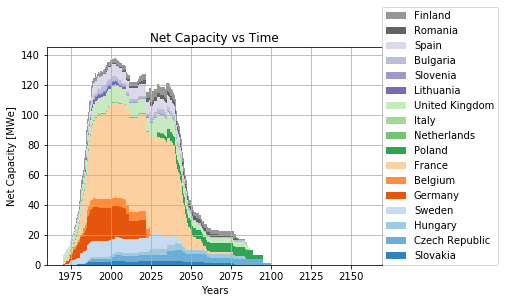
\includegraphics[scale=0.7]{./images/eu_future/power_plot.png}
	\end{center}
	\caption{The timeseries of installed nuclear capacity in the EU are separated by \texttt{Region}s in \Cyclus.
			 The sudden drops in capacity are caused by nuclear phaseout plans by nations like Germany and Belgium.
             The predictions into the future are made to the farthest planed future.
			 }
	\label{fig:eu_pow}
\end{figure}

\subsection{French \gls{SFR} Deployment Schedule}

From 2040,
600-MWe \glspl{SFR} are deployed to make up for the 
decommissioned \gls{LWR} capacities. 
This results in an installed \gls{SFR} capacity of 66,000 MWe
 by 2076, when the last \gls{LWR} decommissions.

\begin{figure}[htbp!]
        \begin{center}
                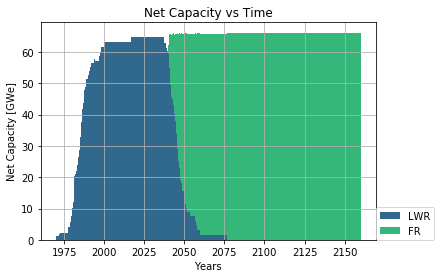
\includegraphics[scale=0.6]{./images/french-transition/power_plot.png}
        \end{center}
        \caption{This plot shows the potential French transition from \glspl{LWR} to \glspl{SFR}.
				 The aggressive growth of nuclear in the 1980s leads to a substantial shutdown
				 of nuclear in the 2040s, which would be replaced by new \glspl{SFR}. The net
				 capacity is kept at a constant of 66 GWe.}
        \label{fig:sfr_num}
\end{figure}
\begin{figure}[htbp!]
	\begin{center}
		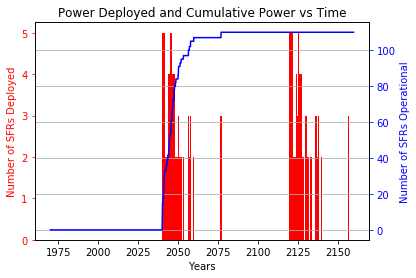
\includegraphics[scale=0.6]{./images/french-transition/sfr_deploy.png}
	\end{center}
	\caption{The deployment of \glspl{SFR} in France is characterized by a period of
		     aggressive building. An average of four reactors are built per year to
		     make up for the decommissioned power plants built in the 1980s and 1990s.
		     The second period of aggressive building occurs when the first generation
		     of \glspl{SFR} decommission after 80 years.}
	\label{fig:dep}
\end{figure}

\begin{figure}[htbp!]
    \begin{center}
        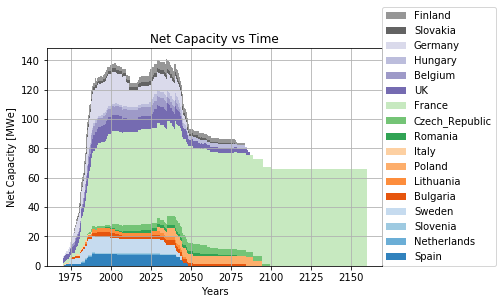
\includegraphics[scale=0.6]{./images/eu_future/onesim.png}
    \end{center}
    \caption{The total deployment scheme of the simulation. The historical
             operation \gls{EU} reactors is followed by the French
             transition to \glspl{SFR}.}
    \label{fig:tot_dep}
\end{figure}


\Cref{fig:sfr_num} and \ref{fig:dep} display
the French transition to \glspl{SFR} over time.
\Cref{fig:tot_dep} displays the total deployment
scheme of the simulation.
The steep transition from 2040 to 2060 reflects the scheduled
decommissioning of reactors built in the 1975-2000
era of aggressive nuclear growth in France.

In reality, building five reactors every year is highly unrealistic. However,
this analysis is to analyze material flow, claiming that, if such an aggressive
deployment scheme was to take place, the \glspl{SFR} would have enough fuel.
More realistically, the deployment of new \glspl{SFR} can be spread out by
staggering scheduled decommissioning of \glspl{LWR} through lifetime extensions.
An analysis of the effect of \gls{LWR} lifetime extension is shown in a later section.


\subsection{Material Definitions}
Depletion calculations of the nuclear fuel are recipe-based, such that a fresh 
and used fuel recipe is defined for each reactor type.
For the compositions of the used fuel, a reference depletion calculation
from ORIGEN is used (see \cref{tab:comp}). The recipe has also been used for
\cite{wilson_adoption_2009}.


\begin{table}[h]
    \centering
%   \scalebox{0.86}{
        \begin{tabular}{cccc}
            \hline
             & \multicolumn{3}{c}{ Composition [\%]} \\
            Recipe & U-235  & U-238  & Pu \\ 
            \hline
            Fresh \gls{UOX} Fuel & 3.1 & 96.9 & -   \\ 
            Fresh \gls{MOX} Fuel & 0.2 & 90.7 & 9.1 \\ 
            Fresh \gls{ASTRID} Fuel & 0.2 & 77.7 & 22 \\
            \hline
        \end{tabular}
        \caption{Fresh fuel compositions used for the simulation \cite{wilson_adoption_2009, varaine_pre-conceptual_2012}.}
        \label{tab:sim_result}
\end {table}


\subsection{Material Flow}
The simulated fuel cycle is illustrated in \cref{diag:fc}.
A source provides natural uranium, which is enriched by an enrichment
facility to produce \gls{UOX}, while disposing enrichment waste (tails)
to the sink. The enriched \gls{UOX} fuels
the \gls{LWR}s and \gls{UOX} waste is produced. The used fuel
is sent to a pool to cool for 3 years \cite{carre_overview_2009}.
The cooled fuel is then reprocessed to separate plutonium and uranium,
or sent to a repository.
The plutonium mixed with depleted uranium (tails) makes \gls{MOX}.
Reprocessed uranium is unused and stockpiled. Uranium is reprocessed
in order to separate the raffinate (Minor actinides and fission products)
from `usable' material. Though neglected in this paper, reprocessed
uranium may substitute depleted uranium for \gls{MOX} production. In the
simulations, sufficient depleted uranium existed that using reprocessed
uranium was overlooked. However, further in the future where the depleted
uranium inventory drains, reprocessed uranium (or, natural uranium) will need to be utilized. 


% Define block styles
\tikzstyle{decision} = [diamond, draw, fill=blue!20, 
text width=4.5em, text badly centered, node distance=3cm, inner sep=0pt]
\tikzstyle{block} = [rectangle, draw, fill=blue!20, 
text width=5em, text centered, rounded corners, minimum height=4em]
\tikzstyle{line} = [draw, -latex']
\tikzstyle{cloud} = [draw, ellipse,fill=red!20, node distance=3cm,
minimum height=2em]


\begin{figure}
        \centering
        \scalebox{0.7}{
                \begin{tikzpicture}[align=center, node distance = 3cm and 3cm, auto]
                % Place nodes
                \node [block] (sr) {Mine (\texttt{SOURCE})};
                \node [cloud, below of=sr] (nu) {Nat U};
                \node [block, below of=nu] (enr) {Enrichment ({\footnotesize \texttt{ENRICHMENT}})};
                \node [cloud, below of=enr] (uox) {\gls{UOX}};
                \node [block, below of=uox] (lwr) {\gls{LWR} (\texttt{REACTOR})};
                \node [cloud, right of=lwr] (snf) {\gls{UNF}};
                \node [cloud, right of=uox] (cunf) {Cooled \gls{UNF}};
                \node [block, right of=snf] (pool) {Pool (\texttt{Storage})};
                \node [cloud, left of=lwr] (tl2) {Dep U};
                \node [cloud, right of=enr] (tl) {Dep U};
                \node [block, right of=tl] (sk) {Repository (\texttt{SINK})};
                \node [cloud, below of=pool] (cunf2) {Cooled \gls{UNF}};
                \node [block, below of=snf] (rep) {{\small Reprocessing ({\footnotesize \texttt{SEPARATIONS}})}};
                \node [cloud, below of=rep] (u) {Sep. U} ;
                \node [cloud, left of=rep] (pu) {Sep. Pu};
                \node [block, left of=pu] (mix) {Fabrication (\texttt{MIXER})};
                \node [cloud, below of=mix] (mox) {\gls{MOX}};
                \node [block, below of=mox] (mxr) {\gls{MOX} Reactors};
                \node [cloud, right of= mxr] (snmox) {Spent \gls{MOX}};
                
                \draw[->, thick] (sr) -- (nu);
                \draw[->, thick] (nu) -- (enr);
                \draw[->, thick] (enr) -- (tl);
                \draw[->, thick] (enr) -- (tl2);
                \draw[->, thick] (tl) -- (sk);
                \draw[->, thick] (tl2) -- (mix);
                \draw[->, thick] (enr) -- (uox);
                \draw[->, thick] (uox) -- (lwr);
                \draw[->, thick] (lwr) -- (snf);
                
                \draw[->, thick] (lwr) -- (snf);
                \draw[->, thick] (snf) -- (pool);
                \draw[->, thick] (pool) -- (cunf);
                \draw[->, thick] (pool) -- (cunf2);
                \draw[->, thick] (cunf) -- (sk);
                \draw[->, thick] (cunf2) -- (rep);
                
                \draw[->, thick] (rep) -- (u);
                \draw[->, thick] (rep) -- (pu);
                \draw[->, thick] (pu) -- (mix);
                \draw[->, thick] (mix) -- (mox);
                \draw[->, thick] (mox) -- (mxr);
                \draw[->, thick] (mxr) -- (snmox);
                \draw[->, thick] (snmox) -- (rep);
                
                \end{tikzpicture}
        
                }
                \caption{The blue boxes represent fuel cycle facilities, and the red ovals
	                	 represent materials. The facility names in parenthesis are archetype names
	                	 used in \Cyclus. \gls{MOX} Reactors include both French \glspl{PWR} and
	                	 \glspl{SFR}.}
                \label{diag:fc}
\end{figure}
\FloatBarrier
